\chapter{The Interaction of Selection, Mutation, and Migration.}
\label{Chapter:Sel_Mut_Mig}

Genetic variation is the raw fuel of evolution. Without variation,
natural selection would have nothing to act on to shape adaptive traits.
However, variation can be deleterious.

Mutation,
broadly defined, is the ultimate source of all genetic
variation and is constantly introducing new variation into all
populations. However, mutation is random and so mutations
that affect function are often damaging. Thus mutation will, in the absence of
sufficiently strong selection, degrade pre-existing adaptations and
undo the work of selection that has built up functional regions of DNA over time. 


Migration, the movement of individuals into a population,
can also increase variation to the population as the individuals
bring new alleles in from surrounding populations. Thus migration can
be an important source of adaptive alleles, aiding their spread
amongst populations within a species. Adaptive alleles can 
introgression between species if low levels of interbreeding occur.
They can sometimes spread between very diverged clades of species, indeed sometimes different domains of life, thanks to horizontal gene
transfer. However, again, just like mutation, migration can disrupt
adaptations. When populations are locally adapted migration amongst
populations can introduce maladaptive alleles into well adapted
populations. If this migration pressure is sufficiently strong, it can lead to the collapse of local
adaptations, or even the collapse of species. 

In this chapter we'll study some of the interplay between selection,
migration, and mutation. 

\subsection{Mutation--Selection Balance}
%</source-file>
Mutation is constantly introducing new alleles into the
population. Therefore, variation can be maintained within a
population not only if selection is balancing (e.g.\ through heterozygote advantage or fluctuating selection over time, as we have seen in the previous section), but also due to a balance between
mutation introducing deleterious alleles and selection acting to purge
these alleles from the population \citep{Haldane:37}. To study mutation-selection balance, we return to the model of directional selection, where allele $A_1$ is advantageous, i.e.
\begin{center}
\begin{tabular}{lccc}
genotype & $A_1A_1$ & $A_1A_2$ & $A_2A_2$ \\
absolute fitness & $W_{11}$ & $ \geq W_{12} \geq$ & $W_{22}$ \\
relative fitness & $w_{11}=1$ & $w_{12}=1-sh$ & $w_{22}=1-s$. \\
\end{tabular}\\
\end{center}
We'll begin by considering the case where allele $A_2$ is not
completely recessive ($h>0$), so that the heterozygotes suffer at least some disadvantage. We denote by $\mu = \mu_{1\rightarrow2}$ the  mutation rate per generation from $A_1$ to the deleterious allele $A_2$, and assume that there is no reverse mutation ($\mu_{2\rightarrow1} = 0$).  Let us assume that selection against $A_2$ is relatively strong compared to the mutation rate, so that it is justified to assume that $A_2$ is always rare, i.e.\ $q_t = 1-p_t \ll 1$. Compared to previous sections, for mathematical clarity, we also switch from following the frequency $p_t$ of $A_1$ to following the frequency $q_t$ of $A_2$. Of course, this is without loss of generality. The change in frequency of $A_2$ due to selection can be written as
\begin{equation}
	\Delta_S q_t = \frac{ \wbar_2 - \wbar_1}{\wbar} p_t q_t  \approx  -hs q_t.
	\label{eq:dirSelApprox}
\end{equation}
This approximation can be found by assuming that $q^2 \approx 0$, $p \approx 1$,
and that $\wbar \approx w_1$. \sa{All of these assumptions make sense if $q \ll 1$. From eqn.\ \eqref{eq:dirSelApprox} we see that selection acts to reduce the frequency of $A_2$ (as both $h$ and $s$ are positive), and it does so geometrically across the
generations. That is, if the initial frequency of $A_2$ is $q_0$, then its frequency at time $t$ is approximately 
\begin{equation}
	q_t = q_0 (1 - hs)^t.
	\label{eq:dirSelExplApprox}
\end{equation}

We will now consider the change in frequency induced by mutation. Recalling that $\mu$ is
the mutation rate from $A_1$ to $A_2$ per generation, the frequency of $A_2$ after mutation is
\begin{equation}
	q^{\prime} =  \mu p_t + q_t = \mu(1 - q_t) + q_t.
\end{equation}
Assuming that $\mu \ll 1$ and that $q \ll 1$, the change in the
frequency of allele $A_2$ due to mutation ($\Delta_M q_t$) can be approximated by
\begin{equation}
	\Delta_M q_t = q^{\prime} - q_t =  \mu.
	\label{eq:mutApprox}
\end{equation}
Hence, when $A_2$ is rare and the mutation rate is low, mutation acts to linearly increase the frequency of the deleterious allele $A_2$.\\

If selection is to balance deleterious mutation, their combined effect over one generation has to be zero. Therefore, to find the mutation--selection equilibrium, we set
\begin{equation}
	\Delta_M q_t + \Delta_S q_t = 0,
\end{equation}
insert eqns. \eqref{eq:dirSelApprox} and \eqref{eq:mutApprox}, and solve for $q$ to obtain
\begin{equation}
	q_e = q_t = \frac{\mu}{hs}.
	\label{eqn:mut_sel_bal}
\end{equation}
We see that the frequency of the deleterious allele $A_2$ is balanced at a frequency equal to the mutation rate ($\mu$) divided by
the reduction in relative fitness in the heterozygote ($hs$).}\\

It is worth pointing out that the fitness of the $A_2A_2$ homozygote
has not entered this calculation, as $A_2$ is so rare that it is hardly ever found in the 
homozygous state. Therefore, if $A_2$ has any deleterious effect
in a heterozygous state (i.e.\ if $h>0$), it is this effect that determines the
frequency at which $A_2$ is maintained in the population. Also, note that by
writing the total change in allele frequency as $\Delta_M q_t + \Delta_S q_t
$ we have implicitly assumed that we can ignore terms of order $\mu
\times s$. That is, we have assumed that mutation and selection are
both relatively weak. This assumption is valid under our prior assumption that both $\mu$ and $s$ are small.\\


If an allele is truly recessive (although few likely are), we have $h=0$, and
so eqn.\ \eqref{eqn:mut_sel_bal} is not valid. However, we can make an argument similar to the one above to show
that, for truly recessive alleles,
\begin{equation}
	q_e = \sqrt{\frac{\mu}{s}}. \label{eqn:recess_mut_sel_bal} 
\end{equation}
\graham{Add figure illustrating the freq as a function of h and s}
\begin{marginfigure}
\begin{center}
  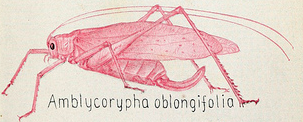
\includegraphics[width = \textwidth]{Journal_figs/single_locus_selection/mutation_selection_balance/Pink_Katydid.png}
\end{center}
\caption{Oblong-winged katydid. \BHLNC{Field book of insects (1918). Lutz,
  F.E. . Illustrations by Edna L. Beutenm\"uller. }{https://www.flickr.com/photos/biodivlibrary/6244366674/in/album-72157627768739853/}{MBLWHOI Library}} \label{fig:katydid}  
\end{marginfigure}
\begin{question}
Oblong-winged katydids ({\it Amblycorypha oblongifolia}) are usually
% these are actually false katydid
green. However, some are bright pink, thanks to an erythrism
mutation (a nice example of early Mendelian reasoning in a wonderfully
titled paper\cite{Wheeler:07}). 
This pink condition is thought to be due to
a dominant mutation (\href{https://blogs.scientificamerican.com/running-ponies/in-north-american-katydids-green-isne28099t-the-dominant-colour-pink-is/}{Crew, 2013}). Assume that roughly  %\citet{Crew:13}
one in ten thousand katydids is bright pink and that the mutation rate at the
gene underlying this condition is $10^{-5}$. What is the relative fitness of heterozygotes for the pink mutation? 
\end{question}

\paragraph{The genetic load of deleterious alleles}
What effect do such deleterious mutations at mutation--selection balance have on the population? It is common to quantify the effect of deleterious alleles in terms of a reduction of the mean relative fitness of the population. For a single site at which a deleterious mutation is segregating at frequency $q_e = \mu/(hs)$, the population mean relative fitness is reduced to
\begin{equation}
	\wbar = 1- 2p_e q_e hs - q_e^2s \approx 1-2\mu.  \label{eqn:mut_load}
\end{equation}
Somewhat remarkably, the drop in mean fitness due to a site segregating
at mutation--selection balance is independent of the selection coefficient against the
heterozygote; it depends only on the mutation rate. Intuitively this is because, given a fixed mutation rate, less deleterious alleles can rise to a higher equilibrium frequency, and thus contribute the same total load as more deleterious (rarer) alleles, but this load is spread across more individuals in the population. Note that this result applies only if the mutation is not totally recessive, i.e.\ if $h > 0$.

A fitness reduction of $2\mu$ is very small, given that the
mutation rate of a gene is likely $<10^{-5}$. However, if there are many loci
segregating at mutation--selection balance, small fitness reductions can accumulate to a substantial so-called
genetic load, a major cause of variation in fitness-related traits
among individuals. For example, the human genome contains over twenty
thousand genes, and many other functional regions, the vast majority
of which will be subject to purifying selection against mutations that
disrupt their function. In humans, most loss of function (LOF) variants, which severely
disrupt a protein-coding gene, are found at low frequencies. However, each human genome typically carries over
a hundred LOF variants \citep{macarthur:12,lek:16}. Not every LOF allele will be
deleterious; some could even be advantageous. However, the combined load of these
LOF alleles must on average lower our fitness, otherwise selection wouldn't be
removing them from the population. Each one of us
carries a unique set of these LOF alleles, usually in a heterozygous state. We differ slightly in how
many of these alleles we carry. For example, the left side of Figure \ref{fig:LOF} shows
the distribution of the number of LOF alleles carried by 769 individuals
of Dutch ancestry. The individuals who carry fewer of these LOF
alleles will on average have higher fitness than those individuals
with more.
\graham{add load for many loci, remember to ref that from BGS section.}


\begin{figure}
\begin{center}
  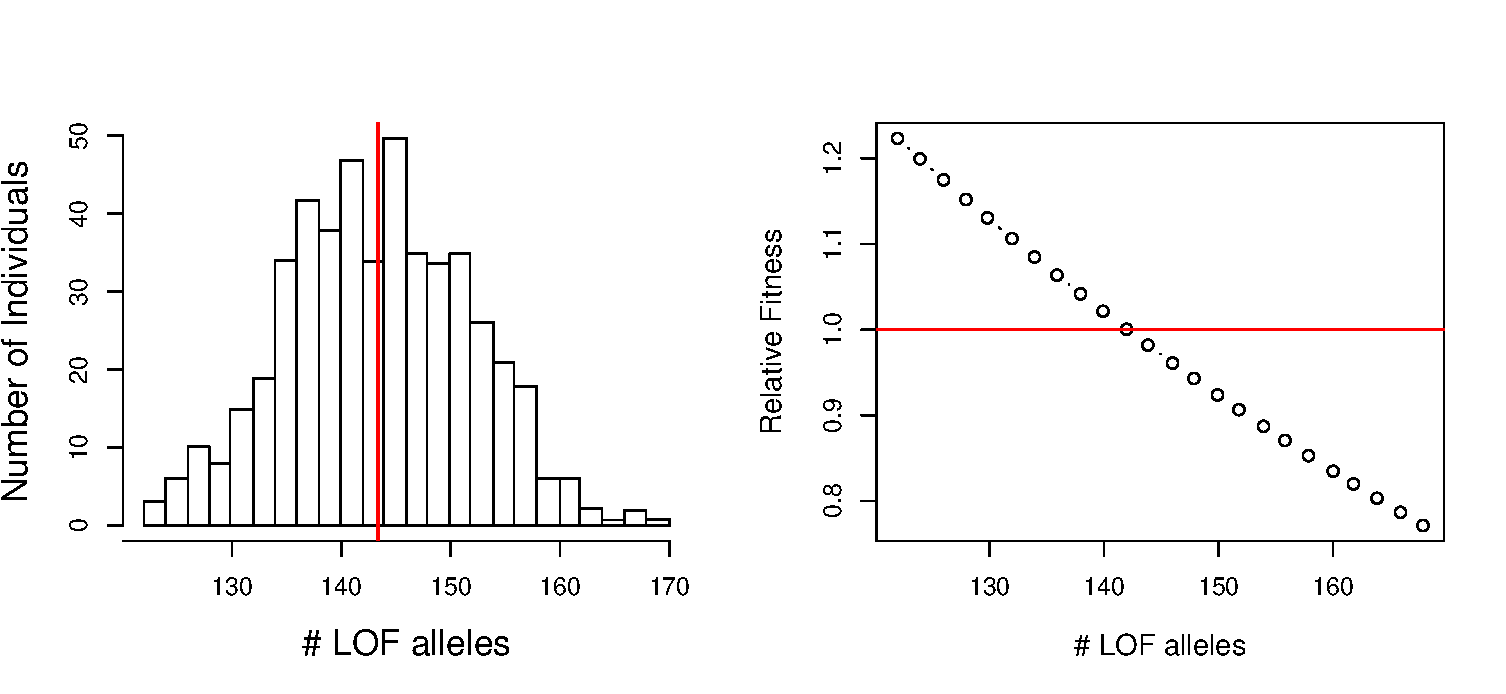
\includegraphics[width = \textwidth]{Journal_figs/single_locus_selection/LOF_variants/Neatherlands_LOF_variants.pdf}
\end{center}
\caption{{\bf Left)} The distribution of LOF alleles in 769 individuals from the
  Genome of the Netherlands project. Data from
  \citeauthor{francioli:14}. The average individual (red line) carries 144 LOF
  alleles. {\bf Right)}. The relative fitness of individuals carrying
  these varying numbers  of LOF alleles, assuming multiplicative
  selection and a selection coefficient of $sh=10^{-2}$ acting against
  these alleles \citep{cassa2017}. \gitcode{https://github.com/cooplab/popgen-notes/blob/master/Journal_figs/single_locus_selection/LOF_variants/Neatherlands_LOF_variants.R}} \label{fig:LOF} 
\end{figure}

How do these differences across individuals in total LOF mutations mount up? Well, if we are willing to assume that the fitness costs of deleterious alleles interact multiplicatively, we can make some
progress. If an individual who carries one LOF mutation has a fitness
$1-hs$,  then an individual who's heterozygote for two LOF mutations would have
fitness $(1-hs)^2$, and an individual who is heterozygote for $L$ LOF
alleles would have fitness  $(1-hs)^L$. The right-hand side of Figure
\ref{fig:LOF} shows the predicted fitness of individuals carrying
varying number of LOF alleles, relative to the mean
fitness of the sample, using this multiplicative model. We don't yet know how much lower the fitness of these
individuals really is, nor do we know how most of these LOF alleles manifest their fitness
consequences through disease and other mechanisms.  However, it's a
reasonable guess that this
variation in LOF alleles, presumably maintained by mutation-selection balance, is
a major source of variation in fitness.


%\begin{question}

%\begin{tcolorbox} 
%\begin{question}
%You are studying an outbred population of mice living in a farmer’s field. Mutations occur at a gene called nurseryrhyme that cause a totally recessive form of blindness. These blind mice do not survive to reproduce as the farmer’s wife cuts off their tail (and other bits) with a carving knife. 
%Surveying the field for baby mice you find that 3 in ten thousand mice are blind.\\
%{\bf A} Assuming that the population mates at random, what is the mutation
% rate of blindness causing alleles?\\
%{\bf B} Following more careful study you now find that there is actually a $20
%\%$ reduction in the viability of heterozygotes for these
%mutations. What would you now estimate as the mutation rate for this
%gene?  
%{\bf C)} Explain how and why your answers differ?
%\end{question}
%\end{tcolorbox}

%B) You look at family of outbred mice. You find that one of the mice in the family is blind, what is the probability that its 1st cousin is also blind?

%C) In another isolated field on the farm, there is a high rate of inbreeding among the mice. The farmer’s wife also carries out her cruel carving knife policy in this field as well. Do you expect to the underlying blindness mutations to be at a higher or low rate in this second field than the first field? Briefly explain your answer.


\subsection{Inbreeding depression}
All else being equal, eqn.\ \eqref{eqn:mut_sel_bal} suggests that mutations that have a smaller effect in the
heterozygote can segregate at higher frequency under mutation--selection balance. As a consequence, alleles that have
strongly deleterious effects in the homozygous state can still segregate at
low frequencies in the population, as long as they do not have too 
strong a deleterious effect in heterozygotes. Thus, outbred populations may have many
alleles with recessive deleterious effects segregating within them.
\begin{question}
Assume that a deleterious allele has a relative fitness $.99$ in
heterozygotes and a relative fitness $0.2$ when present in the
homozygote state. Assume that the
deleterious allele is at a frequency $10^{-3}$ at birth and the
genotype frequencies follow from HWE. Only considering the fitness effects of this locus, and measuring fitness relative to the most fit genotype, answer the following questions: \\
{\bf A)} What is the average fitness of an individual in the population? \\
 {\bf B)} What is the average fitness of the child of a full-sib
 mating? \\
\end{question}
\begin{figure}
\begin{center}
  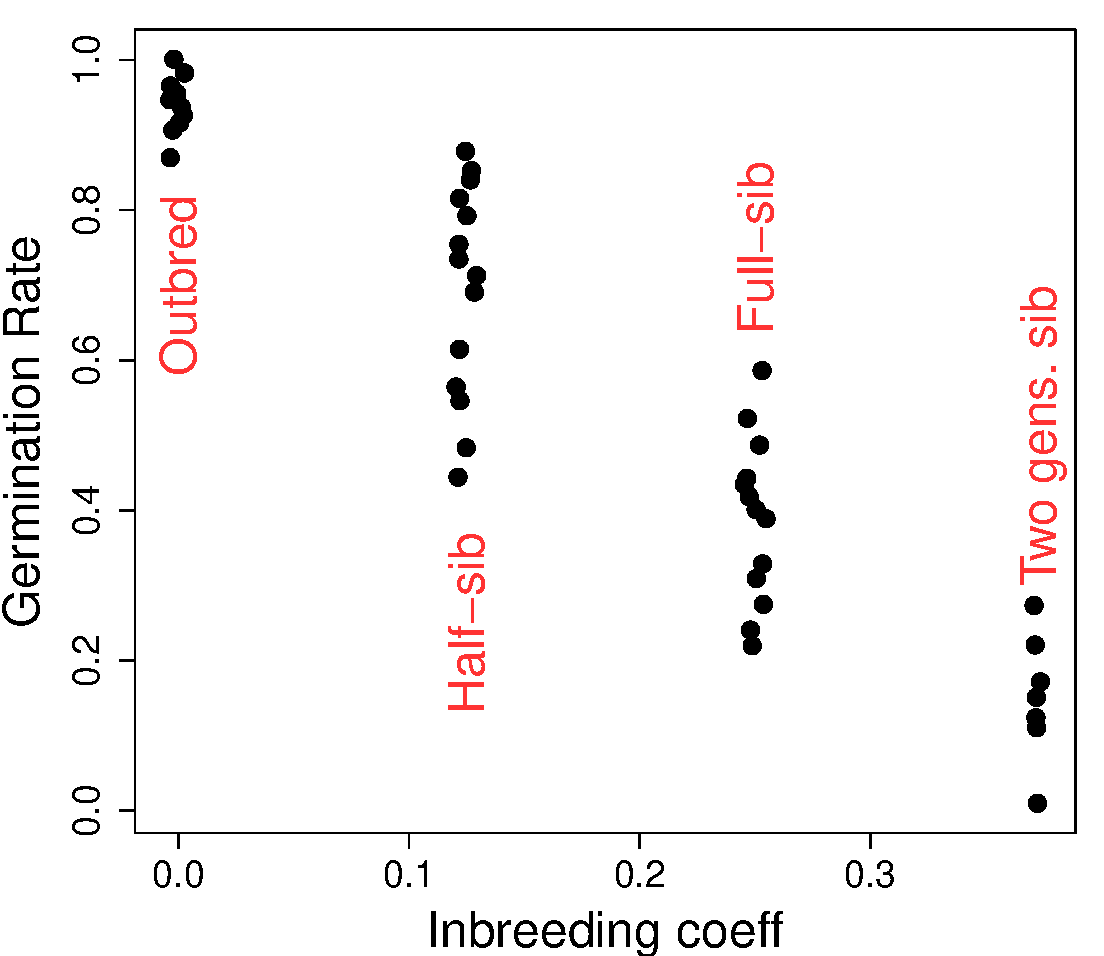
\includegraphics[width = 0.75 \textwidth]{Journal_figs/single_locus_selection/Silene_inbreeding_Richards/Silene_inbreeding_depression.pdf}
\end{center}
\caption{Data showing inbreeding depression over different degrees of
  inbreeding in {\it S. latifolia}. Each point is the mean seed germination rates for different
  family crosses.  Data from \citeauthor{richards:00}. \gitcode{https://github.com/cooplab/popgen-notes/blob/master/Journal_figs/single_locus_selection/Silene_inbreeding_Richards/Silene_inbreeding_depression.R} } \label{fig:Silene_inbreeding} 
\end{figure}

One consequence of segregating for low-frequency recessive deleterious alleles is that inbreeding can reduce fitness.  In typically outbred populations, the mean fitness of individuals
decreases with the inbreeding coefficient, i.e. so-called 'inbreeding depression'
is a common observation. This wide-spread observation dates back to systematic
surveys of inbreeding depression by \citet{darwin:1876}.
Inbreeding depression is likely primarily a consequence of being homozygous at many loci for
alleles with recessive deleterious effects.
\begin{marginfigure}
\begin{center}
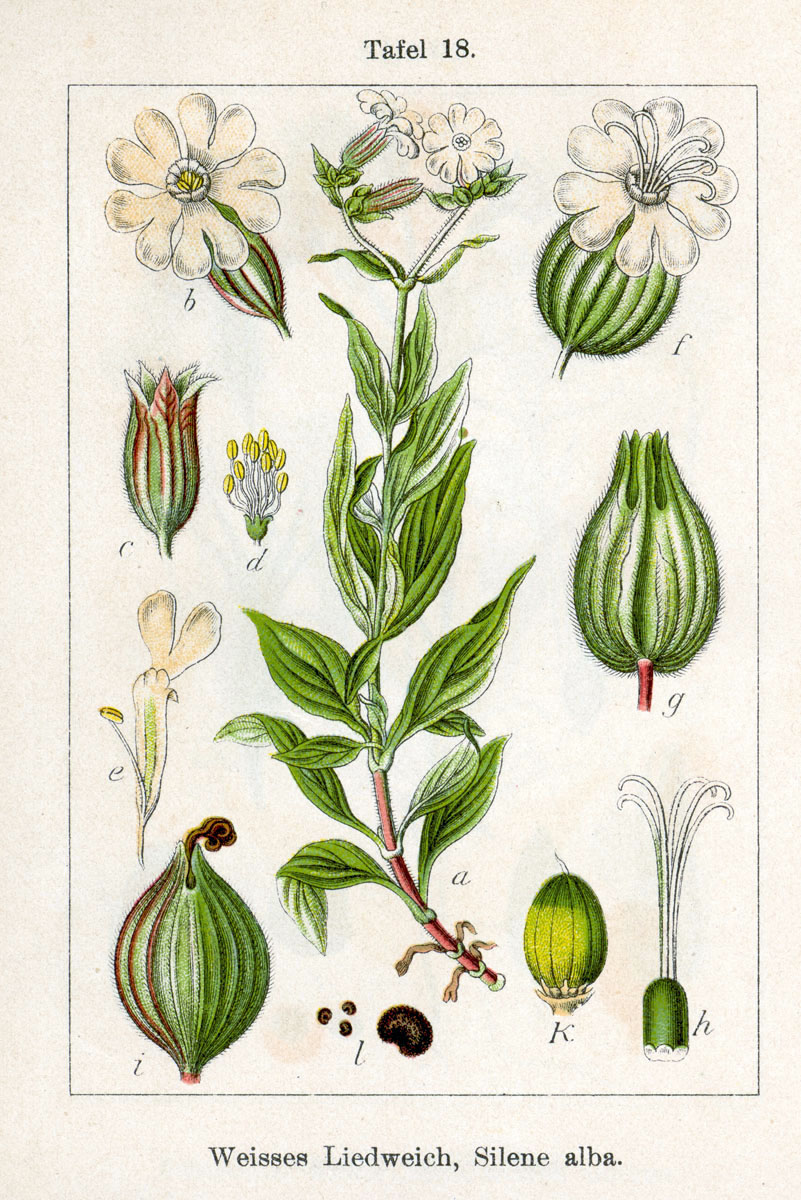
\includegraphics[width = \textwidth]{illustration_images/single_locus_selection/Silene_inbreeding_dep/Silene_latifolia_Sturm18.jpg}
\end{center}
\caption{  White
campion  ({\it S. latifolia}). \newline \noindent \tiny{ Deutschlands Flora in Abbildungen
(1796). Johann Georg Sturm (Painter: Jacob Sturm).  Public Domain,
    \href{https://zh.wikipedia.org/wiki/File:Silene_latifolia_Sturm18.jpg}{wikimedia}.} } \label{fig:Silene} 
\end{marginfigure}

One example of inbreeding
depression is shown in Figure \ref{fig:Silene_inbreeding}.  White
campion ({\it Silene latifolia}) is a dioecious flowering plant; dioecious means that the males and females are
separate individuals. \citeauthor{richards:00} performed crosses to
create offspring who were outbred, the offspring of half-sibs,
full-sibs, and of two generations of full-sib mating. He measured
their germination success, which is plotted in Figure
\ref{fig:Silene_inbreeding}. Note how the fitness of individuals
declines with increased inbreeding. 

\graham{Add decode figure?}

\graham{Add discussion of human inbreeding, and fact that culturally
  we place too much emphasis on ill effects}

\graham{``I do not think anything in my scientific life has given me so much satisfaction as making out the meaning of the structure of heterostylous flowers''.-Darwin}


\paragraph{Purging the inbreeding load.}
Populations that regularly inbreed over sustained periods of time
are expected to partially purge this load of deleterious
alleles. This is because such populations have exposed many of these alleles
in a homozygous state, and so selection can more readily remove these alleles
from the population.

If the population has sustained inbreeding, such that individuals in the population have an inbreeding
coefficient $F$, deleterious alleles at each locus will find a
new equilibrium frequency. Assuming the mutation-selection
model, now with inbreeding, the equilibrium frequency is 
\begin{equation}
	q_e = \frac{\mu}{\big( h(1-F) + F \big) s}
\end{equation}
The frequency of the deleterious allele is decreased due to
the allele now being expressed in homozygotes, and therefore exposed
to selection, more often due to inbreeding.  Thus, all else being equal,
populations with a high degree of inbreeding will purge their load. 
\graham{Add plant eg of purging}
\subsection{Migration--selection balance}
Another reason for the persistence of deleterious alleles in a
population is that there is a constant influx of maladaptive alleles
from other populations where these alleles are locally adaptive.
Migration--selection balance seems unlikely to be as broad an explanation for the
persistence of deleterious alleles genome-wide as mutation-selection
balance. However, a brief discussion of such alleles is worthwhile, as
it helps to inform our ideas about local adaptation.\\


\begin{marginfigure}
\begin{center}
  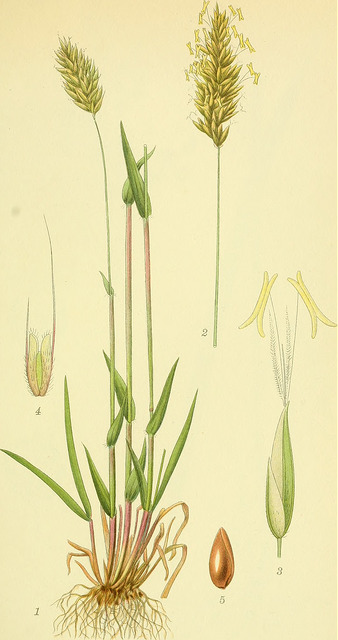
\includegraphics[width = \textwidth]{illustration_images/single_locus_selection/Anthoxanthum_odoratum/19750531053_28f0b3b36e_z.jpg}
\end{center}
\caption{Sweet vernal grass ({\it Anthoxanthum odoratum}). \BHLNC{Billeder af
  nordens flora  (1917).  Mentz, A \& Ostenfeld, C H.}{https://www.flickr.com/photos/internetarchivebookimages/19750531053/in/photolist-wNFPcF-oeKFoD-oeqVrq-xjVkoi-xi5Y8c-whqJ7q-wEuf4k-wJ17N5-tomD7h-wJMXfh-xjM43c-u5erAM-xz2zWL-wH6Dsj-xhwUay-tB85tk-owe1TX-xzu6yj-x4Z1QU-xKkAg9-wR4LKK-xuCehm-xrBNQo-wHELGB-xmTvij-xkqKLC-xzu78f-wCuhJH-x4qfEM-x4p98v-x4n2fg-x3ZDt3-xkAEUP-womZdZ-woh4Wg-x3eR9U-wnUSax-xj2vfv-xf1qFH-x5g4HL-x6c1k4-x4pCYH-w6hCMt-wYM1uh-wZSoKj-w4AuK3-tn7aso-tyRsGC-tiuGr3-ow8wYz}{New York Botanical Garden}} \label{fig:Zinc_plant} 
\end{marginfigure}

Local adaptation \erin{do you need to define local adaptation here?} can occur over a range of geographic scales. Local
adaptation is relatively unimpeded by migration at broad
geographically scales, where selection pressures change more slowly than distances
over which individuals typically migrate over a number of
generations. Adaptation can, however, potentially occur on much finer geographic scales,
from kilometers down to meters in some species. On such small scales,
dispersal is surely rapidly moving alleles between environments, but
local adaptation is maintained by the continued action of selection. An
example of adaptation at fine-scales is shown in Figure
\ref{fig:Zinc_mine} \graham{Fix axis on graph}. \citet{jain1966evolutionary}
studied the patterns of heavy-metal resistance in plants
on mine tailings and in nearby meadows, a set of classic studies of population differences maintained by local adaptation to different soils.
\begin{figure}
\begin{center}
  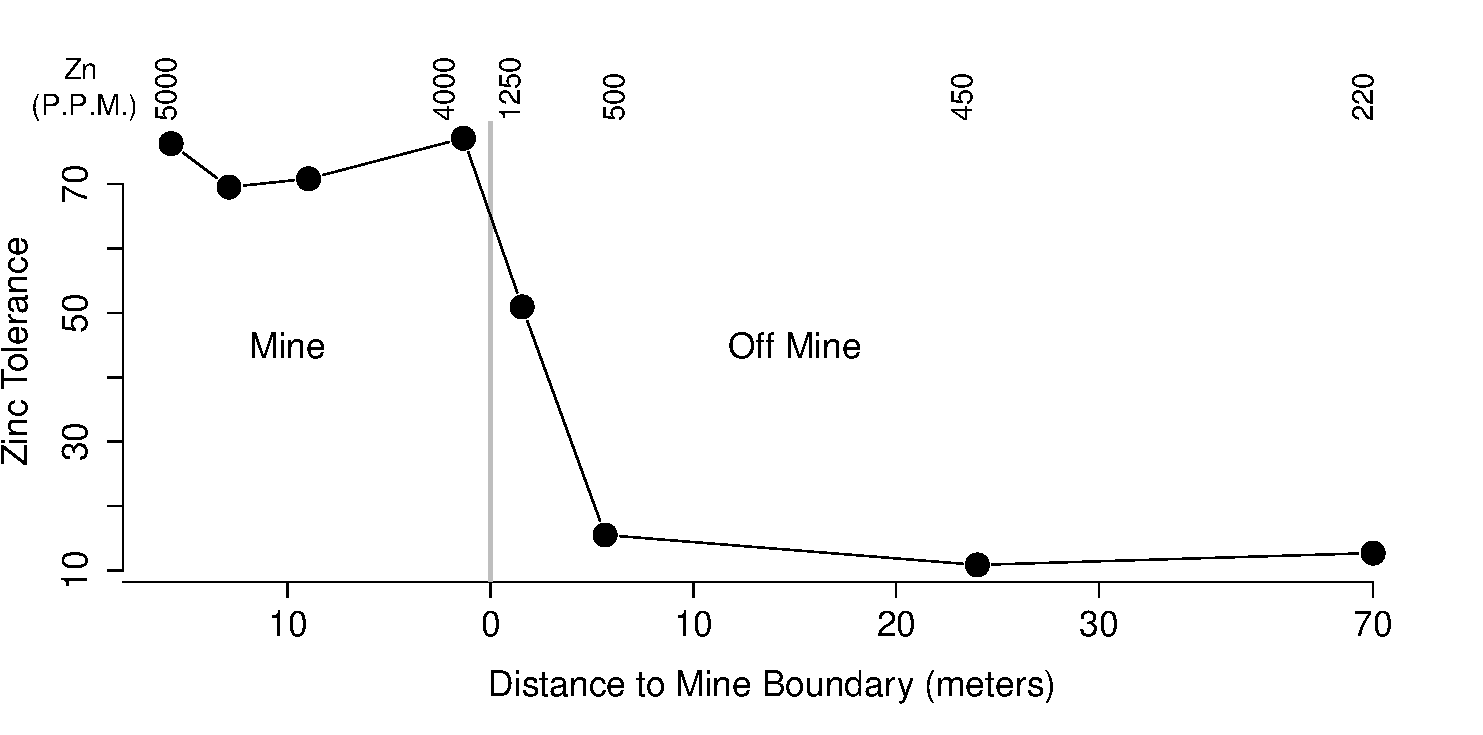
\includegraphics[width = \textwidth]{Journal_figs/single_locus_selection/Anthoxanthum_mines_Jain_Bradshaw/Anthoxanthum_zinc.pdf}
\end{center}
\caption[][2cm]{Data showing the Zinc tolerance of {\it Anthoxanthum
odoratum} on and off of the Trelogan
Mine, Flintshire, North Wales. The numbers along the top give the soil
contamination of Zinc in 
parts per million.  Data from \citet{jain1966evolutionary}. \gitcode{https://github.com/cooplab/popgen-notes/blob/master/Journal_figs/single_locus_selection/Anthoxanthum_mines_Jain_Bradshaw/Anthoxanthum_zinc_Jain_Bradshaw.R}} \label{fig:Zinc_mine} 
\end{figure}
Even at these very short geographically scales, over which seed and
pollen will definitely move, we see strong local
adaptation. Zinc-intolerant alleles are nearly absent from the mine tailings because they prevent plants from growing on these
zinc-heavy soils; conversely, zinc-tolerant alleles do not spread into the meadow populations,  likely due to some trade-off or fitness cost of zinc-tolerance.

As a first pass at developing a model of local adaptation, let's consider a haploid two-allele model with
two different populations, see Figure \ref{fig:mig_sel_bal}, where the relative fitnesses of our alleles
are as follows
\begin{center}
\begin{tabular}{c|cc}
allele & $1$ & $2$ \\
\hline
population 1 & 1 & 1-s \\
population 2 & 1-s & 1 \\
\end{tabular}
\end{center}
As a simple model of migration, let's suppose within a population a
fraction of $m$ individuals are migrants from the other population,
and $1-m$ individuals are from the same population.\\
\begin{marginfigure}
\begin{center}
  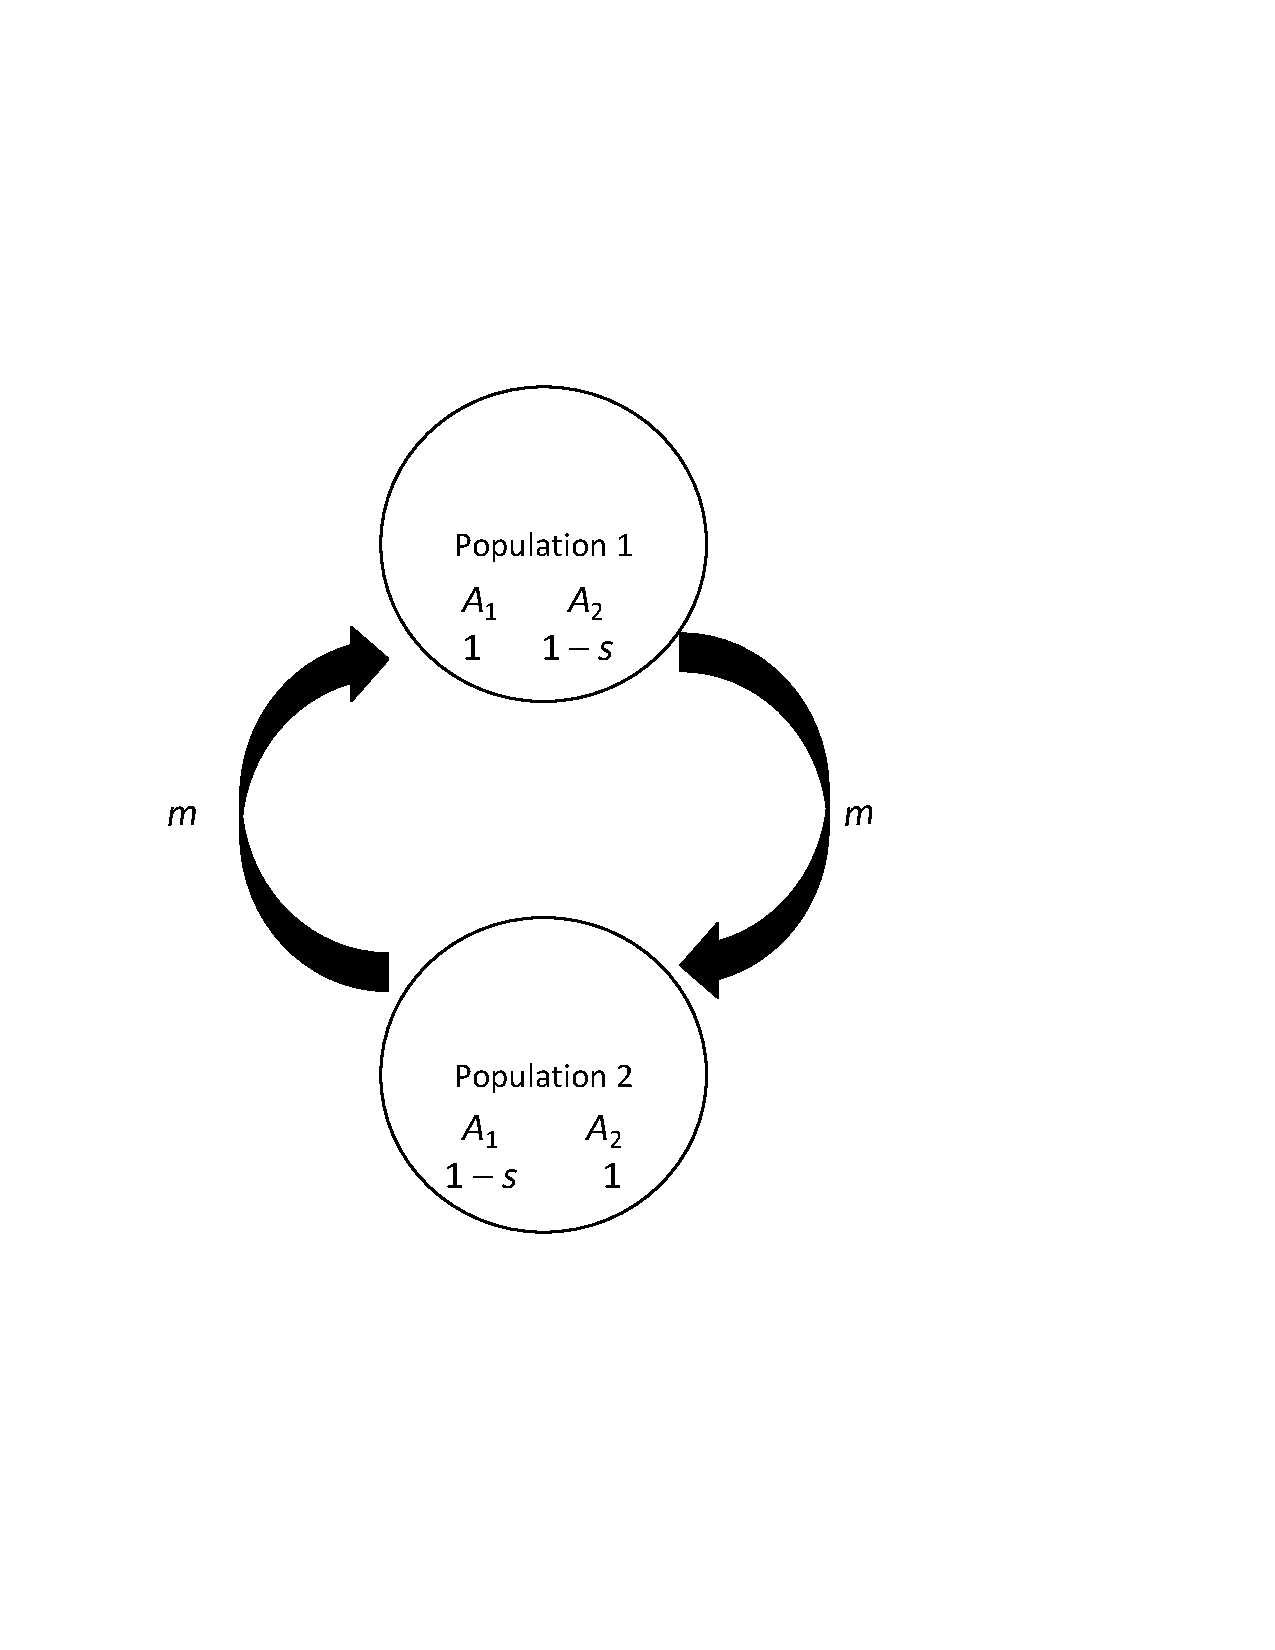
\includegraphics[width = \textwidth]{figures/mig_sel_balance_haploid.pdf}
\end{center}
\caption{Setup of a two-population haploid model of local adaptation.} \label{fig:mig_sel_bal} 
\end{marginfigure}

To quickly sketch an equilibrium solution to this scenario, we'll take an approach analogous
to our mutation-selection balance model. To do this, let's assume that selection is strong compared to migration ($s \gg m$), such that allele
$1$ will be almost fixed in population $1$ and allele $2$ will be
almost fixed in population $2$. If that is the case,
migration changes the frequency of allele $2$ in population $1$ ($q_1$) by
\begin{equation}
\Delta_{Mig.} q_1 \approx m
\end{equation}
while as noted above $\Delta_{S} q_1= -sq_1$, so that migration and
selection are at an equilibrium when $0 = \Delta_{S} q_1+
\Delta_{Mig.}q_1$, i.e. an equilibrium frequency of allele $2$ in
population $1$ of
\begin{equation}
q_{e,1} = \frac{m}{s}
\end{equation}
Here, migration is playing the role of mutation and so
migration--selection balance (at least under strong selection) is
analogous to mutation--selection balance.\\

We can use this same model by analogy for the case of
migration--selection balance in a diploid model. For the diploid case, we replace
our haploid $s$ by the cost to heterozygotes $hs$ from our directional
selection model, resulting in a diploid
migration--selection balance equilibrium frequency of
\begin{equation}
q_{e,1} = \frac{m}{hs} \label{eqn:mig_sel_eq}
\end{equation}

\begin{figure}
\begin{center}
  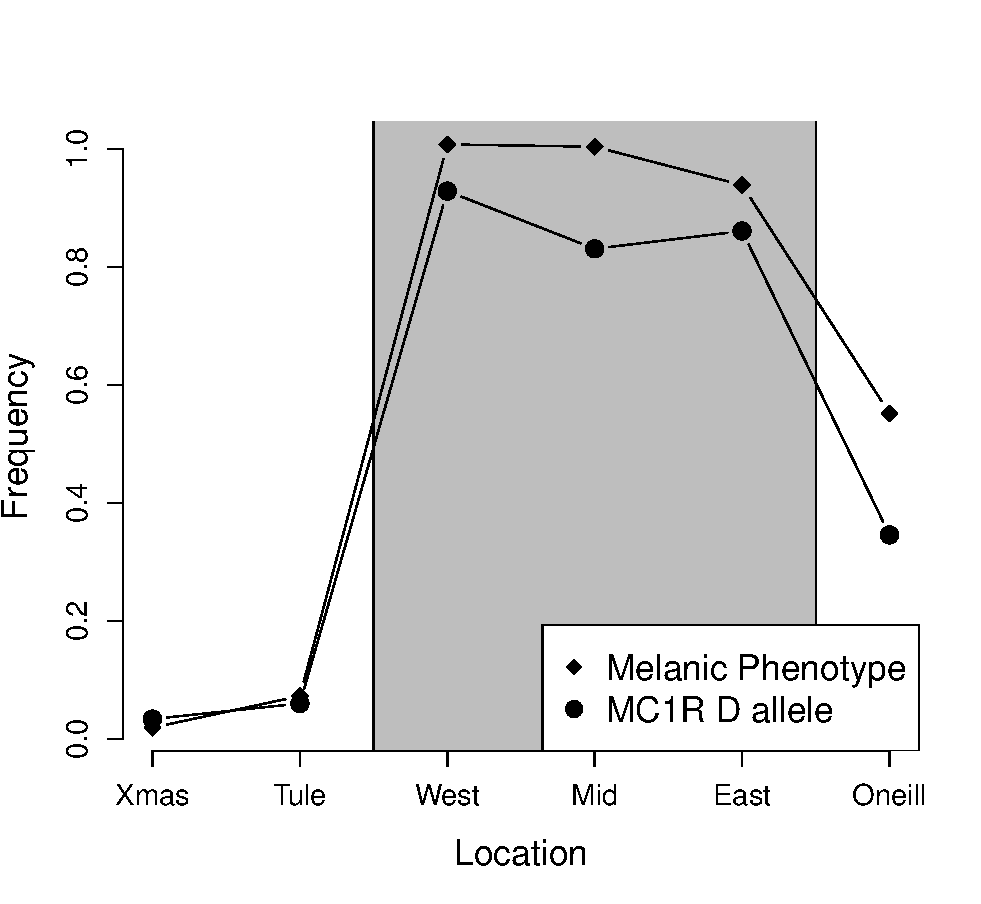
\includegraphics[width = 0.8 \textwidth]{Journal_figs/single_locus_selection/Rock_Pocket_mice/Rock_pocket_mice.pdf}
\end{center}
\caption{Frequency of melanic mice on the lava flow, and at nearby
  locations (diamonds). Frequency of MC1R melanic allele at same
  locations. Data from \citet{hoekstra2004ecological}. \gitcode{https://github.com/cooplab/popgen-notes/blob/master/Journal_figs/single_locus_selection/Rock_Pocket_mice/Rock_pocket_mice.R}} \label{fig:mig_sel_bal_mice} 
\end{figure}

As an example of fine-scale local adaptation due to a single locus,
consider the case of the rock pocket mice adapting to lava flows. Throughout the deserts of the American
Southwest there are old lava flows, where the rocks and soils are much
dark than the surrounding desert. \begin{marginfigure}
\begin{center}
  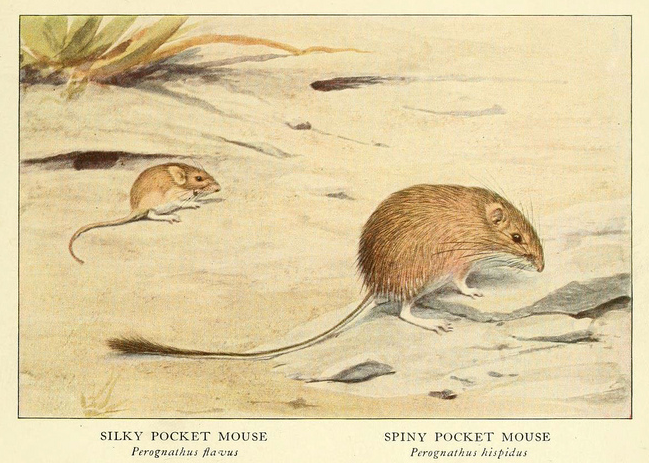
\includegraphics[width =  \textwidth]{illustration_images/single_locus_selection/chaetodipus_pocket_mice/chaetodipus.png}
\end{center}
\caption{Two species from the genus {\it Chaetodipus}, pocket mice,
  formally known as {\it Perognathus}. \BHLNC{Wild animals of North America,
  intimate studies of big and little creatures of the mammal
  kingdom (1918), Nelson, E. W.}{https://www.flickr.com/photos/biodivlibrary/6217227436/in/photolist-x1RbyL-atoV7u-wLxcK5-otRwPb-ovD312-otT7XT-xo6AL1-xXACVH-xWJdrj-x4aerR-w7hgf4-wLxwW3-x5GDbx-x1RehS-w79qy1-x6XU6C-tAuQHM-w7hbgB-wLxXg3-x49K8g-w7hf9g-x71usx-wrkzJ9-oddZ1D-xXADKt-xYfW4F-w8hLZD}{American Museum of Natural History Library}} \label{fig:chaetodipus} 
\end{marginfigure}  Many populations of small animals
that live on these flows have evolved darker pigmentation to be
cryptic against this dark substrate and better avoid visual predators. 
One example of such a locally adapted population are the rock pocket
mice ({\it Chaetodipus intermedius}) who live on the Pinacate
lava flow on the Arizona-Mexico border, studied by
\citet{hoekstra2004ecological}. These mice have much darker, more melanic pelts  than the mice who live on nearby rocky outcrops (see Figure \ref{fig:mig_sel_bal_mice}).   %https://hoekstra.oeb.harvard.edu/files/hoekstra/files/hoekstra2005vol.pdf 
\citet{nachman2003genetic} determined that a dominant allele ($D$) at MC1R
is the primary determinant of this melanic phenotype. The frequency of
this allele across study sites is shown in Figure
\ref{fig:mig_sel_bal_mice}. \citet{hoekstra2004ecological} found that
other, unlinked markers showed little differentiation over these populations, suggesting that the migration rate is high. 

\begin{question}
\citet{hoekstra2004ecological} found that the dark $D$ allele was at
$3\%$ frequency at the Tule Mountains study site. Using $F_{ST}$-based
approaches, for unlinked markers, they estimated that the per individual migration rate was $m=7.0 \times
10^{-4}$ per generation between this site and the  Pinacate lava flow. What is the selection coefficient acting against the dark $D$ allele at the Tule Mountains site? 
\end{question}

%% Selection overrides gene flow to break down maladaptive mimicry https://www.nature.com/articles/nature06532

\paragraph{The width of a genetic cline.}
We can also extend these ideas beyond our discrete model to a model of a population spread out on a landscape where individuals migrate in a more continuous fashion. For simplicity, let's assume a one dimensional
habitat, where the habitat makes a sharp transition in the middle of
our region. You could imagine this to be a set of populations sampled along a
transect through some environmental transition. Our individuals
disperse to live on average $\sigma$ miles away from where they were
born (we can think of this as our individuals migrating a random
distance drawn from a normal distribution, with mean zero, and $\sigma$ being the standard
deviation of this distribution). \marginnote{``Upon an island hard to reach,
the East Beast sits upon his beach.
Upon the west beach sits the West Beast.
Each beach beast thinks he's the best beast.'' --
Theodor Seuss Geisel}. We'll think of a bi-allelic model where
the homozygotes for allele 1 have an additive selective advantage $s$
over allele $2$ homozygotes to the east of our habitat transition (left of
zero in Figure \ref{fig:cline_main}). This flips to allele $2$ having the same advantage $s$ west of the transition (right of zero).  If you've read this send Prof Coop a picture of
the East and West Beast.

\begin{figure}
\begin{center}
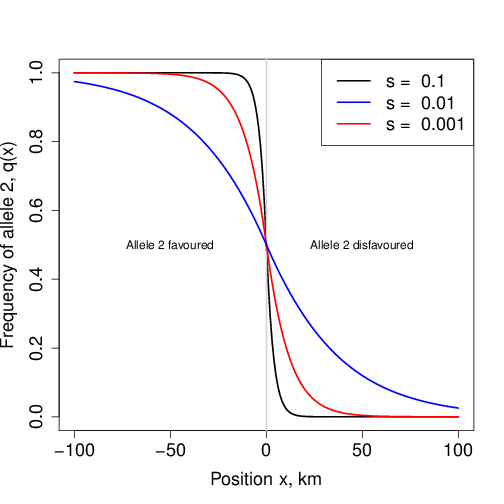
\includegraphics[width=0.7\textwidth]{figures/equilib_cline.png}
\end{center}
\caption{An equilibrium cline in allele frequency (the frequency of
  allele 2, $q(~)$ is shown). Our individuals
  dispersal an average distance of $\sigma=1$miles per generation, and our
allele $2$ has a relative fitness of $1+s$ and $1-s$ on either side of
the environmental change at $x=0$. \gitcode{https://github.com/cooplab/popgen-notes/blob/master/Rcode/cline.R}} \label{fig:cline_main}
\end{figure}

With this setup, we get an equilibrium
distribution of our two alleles, where to the left of zero our allele $2$ is at
higher frequency, while to the right of zero allele $1$ predominates. As we
cross from the left to the right side of our range, the frequency of our allele
$2$ decreases in a smooth cline. The frequency of allele $2$, $q(~)$,
is shown as a function of location along the cline for a variety of
selection coefficients ($s$) in Figure \ref{fig:cline_main}. The width of this cline, i.e. the
geographic distance over which the allele frequency changes, depends on
the relative strengths of dispersal and selection. If selection is
strong compared to dispersal, then selection acts to remove maladaptive
alleles much faster than migration acts to move alleles across the
environmental transition. Thus the allele frequency transition would
be very rapid, and the cline narrow, as we move across the environmental transition. In contrast, if individuals
disperse long distances and selection is weak, many alleles are being moved back and forth over the
environmental transition much faster than selection can act against
these alleles and so the cline would be very wide. 

\begin{marginfigure}
\begin{center}
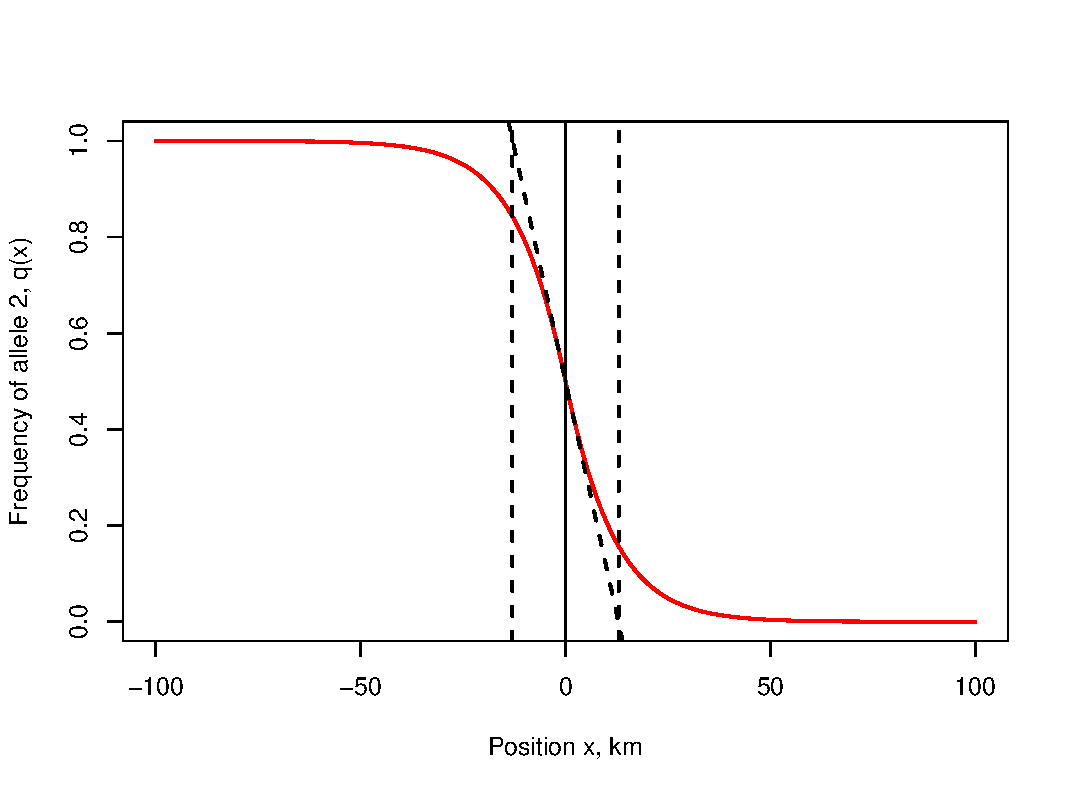
\includegraphics[width=\textwidth]{figures/equilib_width_cline.pdf}
\end{center}
\caption{An equilibrium cline in allele frequency from Figure
  \ref{fig:cline_main}, $s=0.01$. Vertical lines show the cline width. The
  diagonal line show the tangent to the cline at its midpoint. \gitcode{https://github.com/cooplab/popgen-notes/blob/master/Rcode/cline.R}} \label{fig:cline_tangent}
\end{marginfigure}
The width of our cline, i.e. the distance over which we make this shift
from allele $2$ to allele $1$ predominating,
can be defined in a number of different ways. One way to define
the cline width, which is simple to define but perhaps hard to measure
accurately, is via the slope (i.e. the
tangent) of $q(x)$ at $x=0$. See Figure \ref{fig:cline_tangent}. Under this definition, the cline width is
approximately
\begin{equation}
  0.6 \sigma/\sqrt{s} ~\textrm{miles}, \label{eqn:cline_width}
\end{equation}
note that the units are miles here just because we defined the average
dispersal distance ($\sigma$) in miles above. Thus the cline will be wider if individuals dispersal further, higher
$\sigma$, and if selection is weaker, smaller $s$. The appendix below talks through the math underlying these
ideas in more detail.


\begin{figure}
\begin{center}
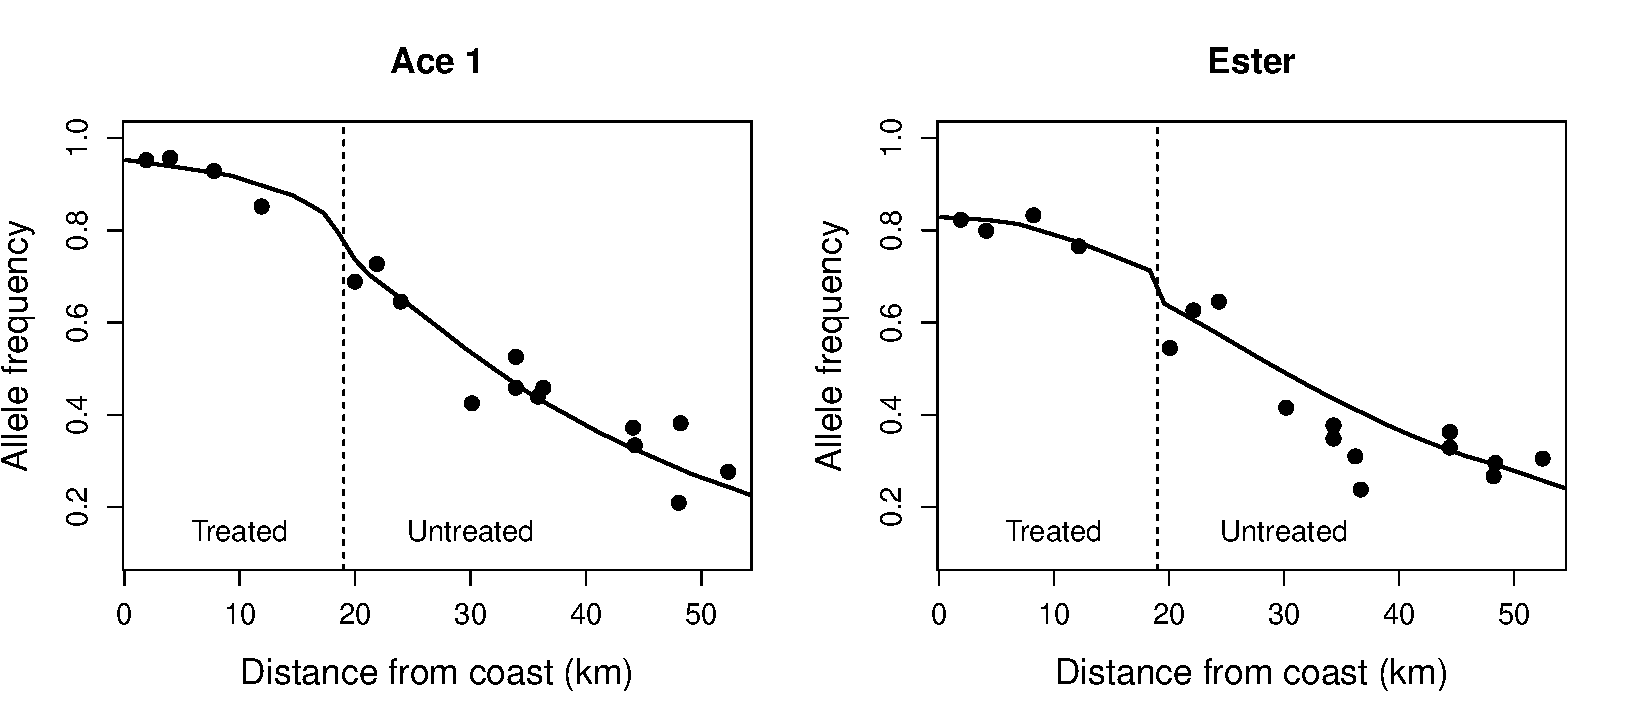
\includegraphics[width=\textwidth]{Journal_figs/single_locus_selection/Culex_resistance/culex_resistance.pdf}
\end{center}
\caption[][-2cm]{Allele frequency clines of two pesticide resistance alleles, at the Ace 1 and Ester genes, in the
  mosquito {\it Culex pipiens}. The dotted line shows where we move from pesticide-treated to untreated
 areas as we move away from the French coast. The dots show observed allele frequencies, the solid lines clines fit under a migration-selection
  balance model of a cline. These allele frequencies represent
 collections over two summers, the frequencies of the alleles are
  substantially reduced in the winter due to the reduced use of
  pesticides. Data from
  \citet{lenormand1999tracking}. \gitcode{https://github.com/cooplab/popgen-notes/blob/master/Journal_figs/single_locus_selection/Culex_resistance/culex_resistance.R}} \label{fig:cline_culex}
\end{figure}


\citet{lenormand1999tracking} collected mosquitoes ({\it Culex pipiens})
in a north–south transect moving away from the Southern French
coast. Areas near the coast were are treated with pesticides, and the mosquitos have
evolved resistance, but areas just a few tens of kilometers from the coast were untreated. \citeauthor{lenormand1999tracking} estimated the frequency
of two unlinked, pesticide-resistance alleles, and found them at high
frequency near the coast but found that their frequencies declined rapidly
moving inland. \citeauthor{lenormand1999tracking} fit migration-selection
cline models to their data, similar to those in Figure \ref{fig:cline_main}, with the pesticide-resistance alleles having an
selection advantage ($s$) in treated areas an a cost ($c$) in untreated areas (they didn't
enforce the selective advantage and cost being symmetric).
\begin{marginfigure}[-3cm]
\begin{center}
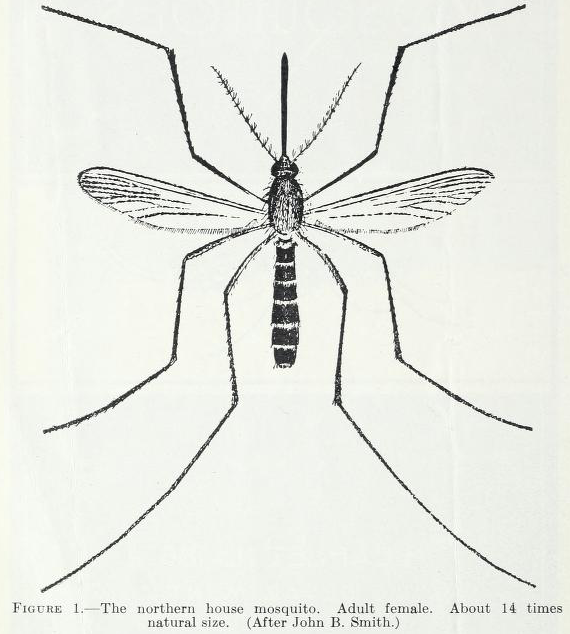
\includegraphics[width=0.7\textwidth]{illustration_images/single_locus_selection/Culex_pipiens/Culex_pipiens.png}
\end{center}
\caption{ mosquito ({\it Culex pipiens}). \BHLNC{Domestic mosquitoes (1939).  Bishopp, F. C.}{https://archive.org/stream/domesticmosquito186bish/\#page/3/mode/1up}{U.S. Department of Agriculture, National Agricultural Library}} \label{fig:culex}
\end{marginfigure}
They
estimated that a higher selective advantage for the Ace 1 allele than
Ester allele ($s=0.33$ and $s=0.19$  respectively) and a higher cost to the Ace 1 allele than
Ester allele in untreated areas ($c=0.11$ and $c=07$
respectively) potentially explaining the less extreme cline for Ester
allele than the  Ace 1 allele. Despite these strong selection pressures we still see a cline
over tens of kilometers because dispersal is relatively high ($\sigma=
6.6$km per generation). 


\paragraph{Hybrid zones}
%https://sci-hub.tw/https://www.nature.com/articles/341497a0
%http://evolution-textbook.org/content/free/figures/18_EVOW_Art/16_EVOW_CH18.jpg
Local adaptation isn't the only way that selection can generate strong
spatial patterns. We can also see strong selection-driven clines when partially-reproductively isolated species spread back in to
secondary contact they can hybridize bringing alleles together
that may not work well with each other. 
One simple model of
is to think about an under-dominant polymorphism, i.e. where the
heterozygote has lower fitness. The two ancestral populations
are alternatively fixed for the two fitter homozygote states,
e.g. ancestral population 1 fixed $A_1A_1$ and ancestral population two the $A_2 A_2$. The
hybrid population forming at the mating edge between the two ancestral populations has a
high frequency of the less fit heterozygotes. Thus hybrids are at a
disadvantage, potentially acting to keep the two populations from
collapsing into each other.  

\begin{figure}
\begin{center}
\includegraphics[width=0.75 \textwidth]{Journal_figs/single_locus_selection/grasshopper_cline_barton_hewitt/grasshopper_cline_barton_hewitt.pdf}
\end{center}
\caption{The frequency of the southern neo-X chromosome moving
  along a valley transect (more southern locations to the right of the
  graph). This represents data from four different
  valleys in the French Alps over less then a kilometer, each point
  represents a sample of 20 males. The red curve is the fitted cline
  under a model of heterozygote disadvantage
  \citep{bazykin1969hypothetical}. Data from
  \citet{barton1981chromosomal},
  \gitcode{https://github.com/cooplab/popgen-notes/blob/master/Journal_figs/single_locus_selection/grasshopper_cline_barton_hewitt/grasshopper_cline_barton_hewitt.R} } \label{fig:grasshopper_cline}
\end{figure}

%% https://commons.wikimedia.org/wiki/File:Brockhaus_and_Efron_Encyclopedic_Dictionary_b56_402-0.jpg
\begin{marginfigure}[1cm]
\begin{center}
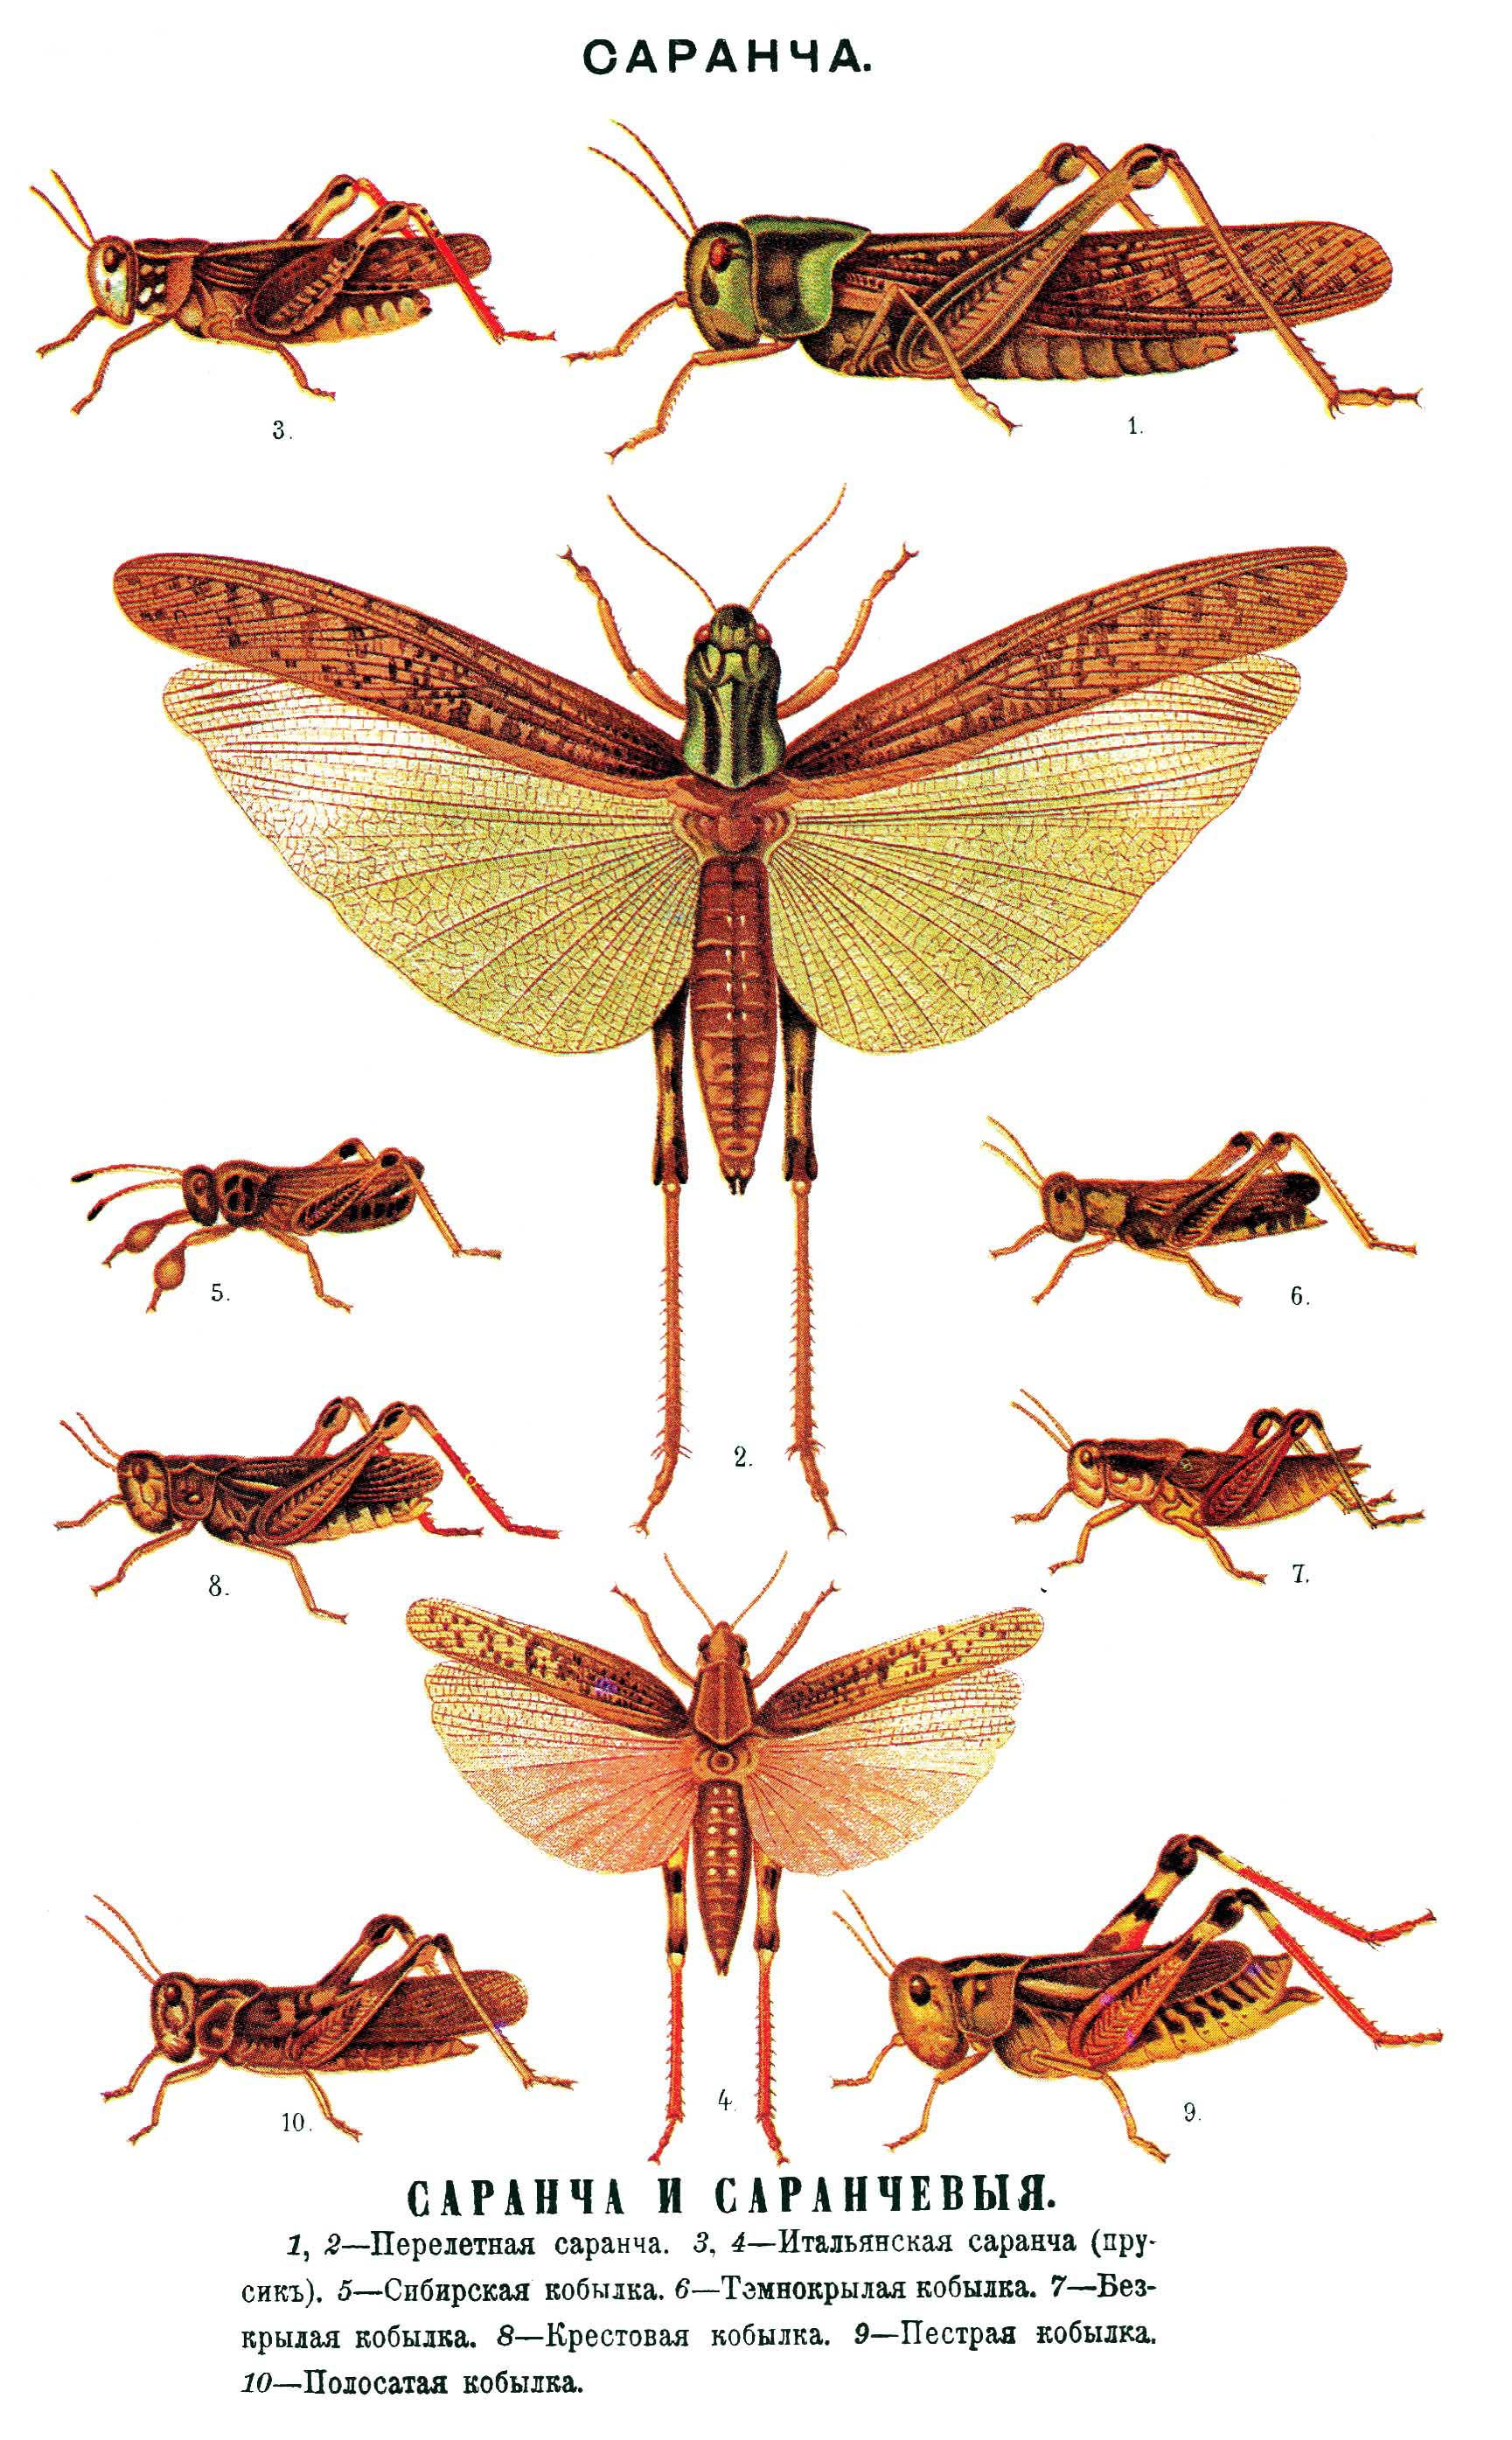
\includegraphics[width= \textwidth]{illustration_images/single_locus_selection/Grasshoppers/634px-Brockhaus_and_Efron_Encyclopedic_Dictionary_b56_402-0.jpg}
\end{center}
\caption{
7. {\it Podisma pedestris}, a species
of short-horned grasshoppers;  from a
page illustrating {\it Orthoptera}.  
\newline \noindent \tiny{Illustration from Brockhaus and Efron
  Encyclopedic Dictionary (1890) Image \href{https://commons.wikimedia.org/wiki/File:Brockhaus_and_Efron_Encyclopedic_Dictionary_b56_402-0.jpg}{wikimedia},  public domain.}
} \label{fig:grasshoppers}
\end{marginfigure}

%Brockhaus and Efron Encyclopedic Dictionary 
Two previously isolated populations of the short-horned grasshopper {\it Podisma pedestris}
have spread into secondary contact in the French Alps, probably after
the last ice age. The population that has spread into the Alps from the south has a large section of novel X chromosome,
due to a chromosomal fusion. This `neo-X' is absent in the populations
that spread from the North into the Alps. The two populations meet in
many valleys running through the Alps, and repeated form a narrow
hybrid zone, with the frequency of the neo-X chromosome forming a very
steep cline transitioning in frequency over a few hundred meters \citep{barton1981chromosomal}.
One potential reason for this steep cline is that females who are
heterozygous for the neo-X (neo-X/old-X) may have reduced fitness, consistent with
an underdominant polymorphism. The neo-X allele cannot spread into the northern
population as it cannot increase in frequency when rate. Conversely
the northern population cannot displace the neo-X, as the old-X is at
a disadvantage.  This spatial distribution at this locus is a tension zone between the
two populations, where neither population can make ground on the other
due to the low fitness of the hybrid.

We can use our same continuous model of migration and selection to
study this setup. Assuming that the homozygotes are equally fit, and
that the heterozygotes relative fitness is reduced by a selection
coefficent $s_h$, the width of the cline is
\begin{equation}
\frac{\sigma}{\sqrt{s_h}}
 \end{equation}
The stronger the selection the more abrupt the transition between the
populations. These wingless grasshoppers move $\sigma \sim 20$ meters
a generation. Thus a reduction in the relative fitness of the hybrid
would be needed to explain this hybrid zone with a width of $\sim
800$m. 

More generally we can see tension zones arise when hybrids have reduced
fitness compared to either species. For example, this can occur due to 
be due to bad epistatic interactions between alleles from each
species. If selection is strong enough on hybrids, often because many
loci are involved in incompatibilities between the species, the entire
genome can be tied up in a tension zone between the two species.  

%Throughout
%most of its range {\it Podisma pedestris} has an X chromosome-based sex
%determination system. But the population



% \begin{question}
% You are investigating a small river population of sticklebacks, which receives infrequent migrants from a very large marine population. At a set of (putatively) neutral biallelic markers the freshwater population has frequencies:\\
% 0.2, 0.7, 0.8\\
% at the same markers the marine population has frequencies:\\
% 0.4, 0.5 and 0.7.\\
%  From studying patterns of heterozygosity at a large collection of markers, you have estimated the long term effective size of your freshwater population is 2000 individuals.\\
% {\bf A)}	What is $F_{ST}$ across these neutral markers in the freshwater population, with respect to the large marine population (i.e. treat the marine population as the total)?\\
% {\bf B)} You are also studying an unlinked locus involved in the
% regulation of salt uptake. In the marine population the ancestral
% allele is at close to fixation, but in your river population the
% derived allele is at 0.99 frequency. Estimate the selective
% disadvantage of the ancestral allele in your river population. [Hint
% how can you use neutral differentiation to estimate the migration rate?]
% \end{question}
 
\subsection*{Appendix: Some theory of the spatial distribution of allele
frequencies under deterministic models of selection}

Imagine a continuous haploid population spread out along a line. Each individual
disperses a random distance $\Delta x$ from its birthplace to the location where
it reproduces, where $\Delta x$ is drawn from the probability density $g(~)$.
To make life simple, we will assume that $g(\Delta x)$ is normally distributed
with mean zero and standard deviation $\sigma$, i.e. migration is unbiased and
individuals migrate an average distance of $\sigma$. \\

The frequency of allele $2$ at time $t$ in the population at spatial location
$x$ is $q(x,t)$. Assuming that only dispersal occurs, how does our allele
frequency change in the next generation? Our allele frequency in the next
generation at location $x$ reflects the migration from different locations in
the proceeding generation. Our population at location $x$ receives a
contribution $g(\Delta x)q(x+\Delta x,t)$ of allele $2$ from the population at
location $x+\Delta x$, such that the frequency of our allele at $x$ in the next
generation is \begin{equation} q(x,t+1) = \int_{-\infty}^{\infty} g(\Delta
x)q(x+\Delta x,t) d \Delta x.  \end{equation}

To obtain $q(x+\Delta x,t)$, let's take a Taylor series expansion of $q(x, t)$:

\begin{equation}
q(x+\Delta x,t) = q(x,t) + \Delta x \frac{dq(x,t)}{dx}+ \tfrac{1}{2}(\Delta x)^2 \frac{d^2q(x,t)}{dx^2}+\cdots
\end{equation}

then

\begin{equation}
q(x,t+1) = q(x,t) +\left( \int_{-\infty}^{\infty} \Delta x g(\Delta x) 
  d \Delta x \right) \frac{dq(x,t)}{dx} + \tfrac{1}{2}\left( \int_{-\infty}^{\infty}(\Delta x)^2 g(\Delta x) 
  d \Delta x \right)  \frac{d^2q(x,t)}{dx^2}+\cdots
\end{equation} 

Because $g(~)$ has a mean of zero, $ \int_{-\infty}^{\infty} \Delta x g(\Delta x) d
\Delta x =0$, and has because  $g(~)$ has variance $\sigma^2$,  $\int_{-\infty}^{\infty}(\Delta
x)^2 g(\Delta x) d \Delta x = \sigma^2 $. All higher order terms in our Taylor series expansion cancel out (as all high moments of the normal distribution are zero). Looking at the change in allele frequency,
$\Delta q(x,t) = q(x,t+1)-q(x,t)$, so

\begin{equation}
\Delta q(x,t) = \frac{\sigma^2}{2} \frac{d^2q(x,t)}{dx^2}
\end{equation} 

This is a diffusion equation, so that migration is acting to smooth out allele frequency differences with a diffusion constant of $\tfrac{\sigma^2}{2}$. This is exactly analogous to the equation
describing how a gas diffuses out to equal density, as both particles in a gas and our individuals of type $2$ are performing Brownian motion (blurring our eyes and seeing time as continuous). \\


We will now introduce fitness differences into our model and set the relative
fitnesses of allele $1$ and $2$ at location $x $ to be $1$ and $1+s\gamma(x)$.
To make progress in this model, we'll have to assume that selection isn't too
strong, i.e. $ s \gamma(x) \ll 1$ for all $x$. The change in
frequency of allele $2$ obtained within a generation due to selection is

\begin{equation}
q^{\prime}(x,t) - q(x,t) \approx s\gamma(x) q(x,t) \big( 1 - q(x,t) \big)
\end{equation}

i.e. logistic growth of our favoured allele at location $x$.  Putting our
selection and migration terms together, we find the total change in allele frequency at location x in one generation is
\begin{equation} q(x,t+1) -
q(x,t) = s\gamma(x) q(x,t) \big( 1 - q(x,t) \big)+\frac{\sigma^2}{2}
\frac{d^2q(x,t)}{dx^2} \label{eqn:fisherKPP} 
\end{equation}
In deriving this result, we
have essentially assumed that migration acted upon our original allele frequencies
before selection, and in doing so have ignored terms of the order of $\sigma s$. 


\begin{figure}
\begin{center}
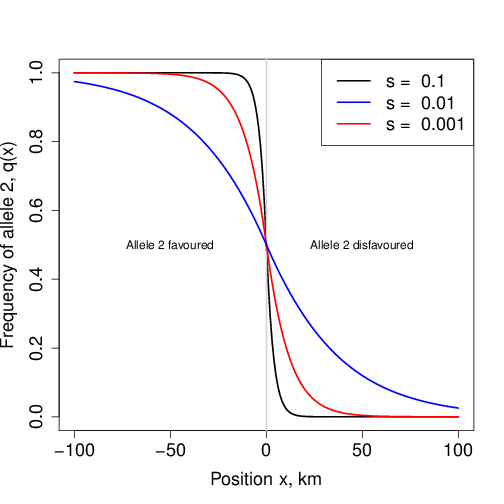
\includegraphics[width=0.5\textwidth]{figures/equilib_cline.png}
\end{center}
\caption{An equilibrium cline in allele frequency. Our individuals
  dispersal an average distance of $\sigma=1$km per generation, and our
allele $2$ has a relative fitness of $1+s$ and $1-s$ on either side of
the environmental change at $x=0$.} \label{fig:cline}
\end{figure}

\paragraph{The cline in allele frequency associated with a sharp
  environmental transition.}
To make progress, let's consider a simple model of local adaptation where the
environment abruptly changes. Specifically, we assume that $\gamma(x)= 1$ for
$x<0$ and $\gamma(x)= -1$ for $x \geq 0$, i.e. our allele $2$ has a selective
advantage at locations to the left of zero, while this allele is at a
disadvantage to the right of zero. In this case we can get an equilibrium
distribution of our two alleles, where to the left of zero our allele $2$ is at
higher frequency, while to the right of zero allele $1$ predominates. As we
cross from the left to the right side of our range, the frequency of our allele
$2$ decreases in a smooth cline. \erin{figure 6.25 is repeating figure 6.24.. }\\



%Under such a model the change in frequency of allele $2$ at location $x$ at time $t$,
%$q(x,t)$, over time follows the differential equation
%\begin{equation}
%\frac{dq(x,t)}{dt} = s\gamma(x) q(x,t) \left( 1 - q(x,t) \right) + \frac{\sigma^2}{2} \frac{d^2q(x,t)}{dx^2}
%\end{equation}
%the first term on the right-hand side is the logistic growth of our
%favoured allele at location $x$, while the second term on the
%right-hand side is the diffusion of allele frequencies due to
%dispersal (i.e. dispersal is acting to spread out the effect of
%allele frequency change across populations). See below for how we
%derive this \gc{to be added}.\\

Our equilibrium spatial distribution of allele frequencies can be found by
setting the left-hand side of eqn. \eqref{eqn:fisherKPP} to zero to arrive at
\begin{equation}
s\gamma(x) q(x) \left( 1 - q(x) \right) = - \frac{\sigma^2}{2} \frac{d^2q(x)}{dx^2}
\end{equation}
We then could solve this differential equation with appropriate boundary
conditions ($q(-\infty)=1$ and $q(\infty) = 0$) to arrive at the
appropriate functional form for our cline. While we won't go into the
solution of this equation here, we can note that by dividing our
distance $x$ by $\ell=\sigma/\sqrt{s}$, we can remove the effect of our
parameters from the above equation. This compound parameter $\ell$ is the characteristic
length of our cline, and it is this parameter which determines over
what geographic scale we change from allele $2$ predominating to
allele $1$ predominating as we move across our environmental shift. \\

%\paragraph{Cline arising from an underdominant polymorphism}

%The width of our cline, i.e. over what distance do we make this shift
%from allele $2$ predominating to allele $1$,
%can be defined in a number of different ways. One simple way to define
%the cline width, which is easy to define but perhaps hard to measure accurately, is the slope (i.e. the
%tangent) of $q(x)$ at $x=0$. Under this definition the cline width is approximately $0.6
%\sigma/\sqrt{s}$.\\

%\paragraph{The rate of spatial spread of a beneficial allele.}
%Consider a beneficial mutation that has arisen in a specific spatial
%location and has begun to spread geographically. 
%\gc{FINISH THIS.}

